\documentclass{Resources/UoBLab1}
\pubyear{2018}
\subjectarea{Computational Vision}
\usepackage{listings}
\usepackage{hyperref}
\usepackage{amsmath}

\begin{document}
\firstpage{1}

\title{Edge Detection}
\author{Charles de Freitas}
\course{Msc Computer Science}
\school{School of Computer Science}
\date{13th December 2018}
\keywords{Filtering, Smoothing}

\maketitle

\begin{abstract}

\end{abstract}


\section{Introduction}
\begin{itemize}
	\item filters
	      \begin{itemize}
	      	\item sobel
	      	\item roberts
	      	\item gaussian
	      	\item laplacian
	      	\item canny
	      \end{itemize}
	\item Smoothing: size, spread
	\item thresholding
\end{itemize}

\section{Theory}
%ENTER THEORY TEXT BELOW
\lipsum[4]

\section{Methods}
\section{Laplacian of Gaussian}
Laplacian of Gaussian refers to convolving a Gaussian smoothing mask with a Laplacian filter.
The Laplacian is a 2-D isotropic measure of the 2nd spatial derivative of an image.\cite{Laplacian}
A small sample laplacian as as follows:
\[
\begin{bmatrix}
    0 & 1 & 0 \\
    1 & 4 & 1 \\
    0 & 1 & 0
\end{bmatrix}
\]

Since MATLAB includes a function for calculcating the discrete laplacian, we can simply perform
\lstinline[language=MATLAB]{del2(img)}\cite{del2}
%ENTER APPARATUS TEXT BELOW


\section{Cell Detection}
\subsection*{Variable Smoothing}
\begin{enumerate}
	\item Create a set of Gaussian masks is produced for each filter.
	\item Create a linear $\Omega$ space bounded by 0 and the largest value possible for a given smoothed image.
	\item Apply the given smoothed filter for $\omega$ where $\omega \in \Omega$
	\item From the resulting set, calculate \textbf{TPR} and \textbf{FPR}.
	\item Repeate for all Gaussians and return a set of coortinates.
	\item Plot the set that contains the shortest distance to \((0,1)\)
	\item Repeate for all filters and respective Gaussians.
\end{enumerate}
\subsubsection*{Tuning}
Since each filter behaves differently, an appropriot set of Gaussian masks must be selected for each.
Starting with fixed values of \begin{math}
\bar{X} = 0 ,  \sigma{} = 1
\end{math}
and a range of
\lstinline[language=MATLAB]{0:1:10}\footnote[1]{From 0 to 10 and stepping by 1}.



\begin{figure}{!hb}
    \begin{center}
		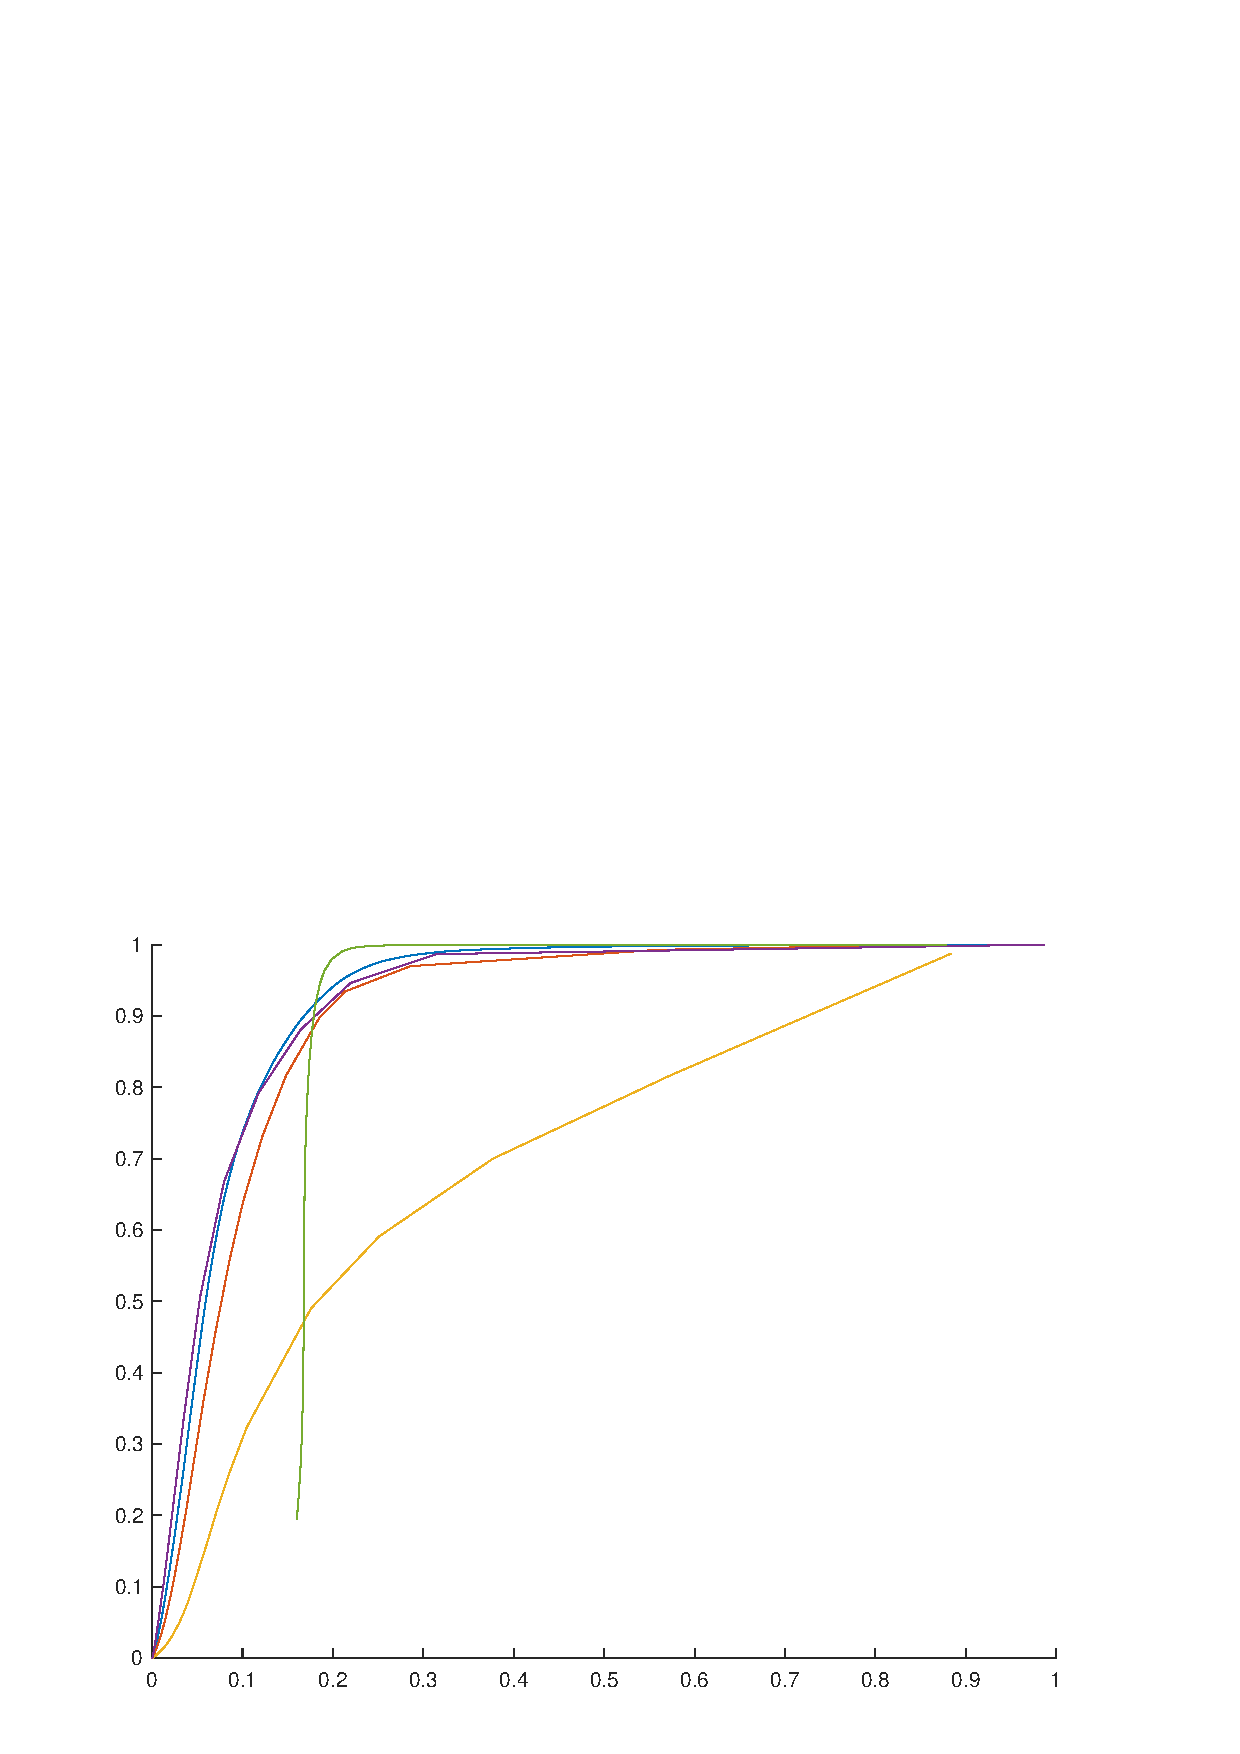
\includegraphics[scale=0.20]{Resources/images/all_1_to_10.jpg}
		\caption{Optimal curves when tested with identical Gaussians of size 0-10}
        \label{fig:1to10}
    \end{center}
\end{figure}



\section{Results}
%ENTER RESULTS TEXT (AND FIGURES) BELOW
\lipsum[7]

\section{Discussion}
\subsection{Analysis}
%ENTER ANALYSIS TEXT BELOW
\lipsum[8]
Something to be cited.\cite{reference2}
\lipsum[2]

\subsection{Validation}
%ENTER VALIDATION TEXT BELOW
\lipsum[9]

\section{Conclusion}
%ENTER CONCLUSION TEXT BELOW
\lipsum[10]

\section*{Acknowledgements}
%ENTER ACKNOWLEDGEMENTS TEXT BELOW
I thank the A for letting me use their equipment and providing access to various research tools, and I thank B, C, and D for discussion and comments on this manuscript.

\begin{thebibliography}{}

    \bibitem{Laplacian}
    \url{https://homepages.inf.ed.ac.uk/rbf/HIPR2/log.htm}
    \bibitem{del2}
    \url{https://uk.mathworks.com/help/matlab/ref/del2.html}
\end{thebibliography}

\end{document}
